\clearpage

\section*{Appendice A. Dispense integrative} \label{appendice-combinatorio}
\markboth{Appendice A. Dispense integrative}{}
\addtocounter{section}{1}
\setcounter{subsection}{0}
\setcounter{teo}{0}
\addcontentsline{toc}{section}{Appendice A. Dispense integrative}
\subsection{Richiami di analisi e insiemistica}\label{analisi-insiemistica}

% Si potrebbero mettere immagini ma sarebbero le stesse delle immagini e controimmagini già usate (o le successioni per l'esempio dei limsup e liminf, ma mi sembra abbastanza inutile) (Fab)
% I concetti sono un po' diversi e andrebbero ripensate bene IMHO. Eviterei. (AW)
\subsubsection{Limite inferiore e superiore}

\begin{defn}
	\index{limite inferiore e superiore!di una successione numerica}
	\index{classe!limite}
	Data una successione $\{x_n\}_{n \in \NN} \subseteq \RR$, sono definiti il \textbf{limite inferiore} e il \textbf{limite superiore} di tale successione:
	$$ \liminf x_n \coloneqq \sup_{n \in \NN} \inf_{k \ge n} x_k = \lim_{n \to +\infty} \inf_{k \ge n} x_k $$
	$$ \limsup x_n \coloneqq \inf_{n \in \NN} \sup_{k \ge n} x_k = \lim_{n \to +\infty} \sup_{k \ge n} x_k$$
	L'intervallo $[\liminf x_n , \limsup x_n]$ è detto \textbf{classe limite} della successione.
\end{defn}
Una successione ammette limite se e solo se $\liminf x_n = \limsup x_n$, ovvero se la classe limite è composta da un solo elemento.
In particolare vale il seguente teorema.

\begin{teo}
	Per qualsiasi successione $\{x_n\}_{n \in \NN}$:
	\begin{enumerate}
		\item il limite inferiore e il limite superiore sono entrambi \emph{unici};
		\item $ \liminf x_n \le \limsup x_n$;
		\item $x_n$ converge o diverge $\iff \liminf x_n = \limsup x_n$.
	\end{enumerate}
\end{teo}

\begin{ese}~\\[-12pt]
	\begin{itemize}	
		\item $x_n = (-1)^n $ ha $ \liminf x_n = -1$ e $ \limsup x_n = 1$, pertanto non ammette limite.
		\item $x_n = \begin{cases}
		1 & \text{se } n \text{ è primo} \\
		0 & \text{altrimenti}
		\end{cases}$ ha $ \liminf x_n = 0$ e $ \limsup x_n = 1$, pertanto non ammette limite.
		\item $x_n = (-n)^n $ ha $ \liminf x_n = -\infty$ e $ \limsup x_n = +\infty$, pertanto non ammette limite.
		\item $x_n = (-\frac{1}{n})^n $ ha $ \liminf x_n = \limsup x_n = 0$ e di conseguenza $\lim_{n}x_n =0$.
		
		
	\end{itemize}
\end{ese}
\needspace{3\baselineskip}
\subsubsection{Operazioni insiemistiche}
\begin{teo}[leggi di De Morgan]
	\index{De Morgan, leggi di}
	Sia $I$ un insieme di indici, anche non numerabile, e sia $\{A_\alpha\}_{\alpha \in I} \subseteq \Omega$ una collezione di insiemi. Allora:
	$$
		\text{1.} \ \left(\bigcup_{\alpha \in I} A_\alpha \right)^C = \bigcap_{\alpha \in I} A_\alpha^C
		\qquad\quad \text{2.} \ \left(\bigcap_{\alpha \in I} A_\alpha \right)^C = \bigcup_{\alpha \in I} A_\alpha^C
	$$
\end{teo}
\begin{dimo}
	\begin{enumerate}
		Per la prima uguaglianza:
		\begin{align*}
		\omega \in \left(\bigcup_{\alpha \in I}A_\alpha \right)^C 
		&\iff \omega \notin \bigcup_{\alpha \in I}A_\alpha & \\
		&\iff \omega \notin A_\alpha \ \forall \alpha \in I & \\
		&\iff \omega \in{A_\alpha}^C \ \forall \alpha \in I & \text{(Complementarità)}\\
		&\iff \omega \in \bigcap_{\alpha}{A_\alpha}^C &
		\end{align*}
	    Per la seconda uguaglianza si procede in maniera analoga. \qedhere
	\end{enumerate}
\end{dimo}

Si esploreranno ora i concetti di immagine e controimmagine.
\begin{defn}
	\index{immagine}
	Data una funzione $X: \Omega \to F$ e un insieme $A \subseteq \Omega$, si dice \textbf{immagine} di $A$ l'insieme
	$X(A) \coloneqq \{x \in E : x = X(\omega), \text{ per qualche }\omega \in A \} \subseteq F$.
\end{defn}

\begin{defn}
	\index{controimmagine}
	Data una funzione $X: \Omega \to F$ e un insieme $B \subseteq F$, si dice \textbf{controimmagine} di $B$ l'insieme
	$X^{-1}(B) = (X \in B) \coloneqq \{ \omega \in \Omega : X(\omega) \in B\} \subseteq \Omega$.
\end{defn}

\begin{teo}
	Data una funzione $X: \Omega \to F$, la controimmagine ha le seguenti proprietà:
	\begin{enumerate}
		\item $X(X^{-1}(B)) \subseteq B \enspace \forall B \subseteq E$;
		\item $X^{-1}(X(A))\supseteq A \enspace \forall A \in \Omega$;
		\item $X^{-1}(B^C)=(X^{-1}(B))^C \enspace \forall B \subseteq E$;
		\item $X^{-1}\left(\bigcup_{\alpha}B_\alpha \right) = \bigcup_{\alpha}X^{-1}(B_\alpha) \enspace
		\forall \{B_\alpha\}_{\alpha \in I} \subseteq E$;
		\item $X^{-1}\left(\bigcap_{\alpha}B_\alpha \right) = \bigcap_{\alpha}X^{-1}(B_\alpha) \enspace
		\forall \{B_\alpha\}_{\alpha \in I} \subseteq E$.
	\end{enumerate}
\end{teo}

\begin{teo}[convergenza puntuale]
	Sia $X_n : \Omega \to \RR$ una successione di funzioni, con $n \in \NN$. Allora:
	\begin{enumerate}
		\item $(\liminf X_n)(\omega) = \liminf \left( X_n(\omega) \right)$;
		\item $(\limsup X_n)(\omega) = \limsup \left( X_n(\omega) \right)$;
		\item Se per ogni $\omega \in \Omega$ fissato $X_n(\omega)$ converge per $n \to +\infty$, allora $(\lim_n X_n)(\omega) = \lim_n \left( X_n(\omega) \right)$.
	\end{enumerate}
\end{teo}
I membri sinistri delle 3 uguaglianze sono da intendersi come una singola funzione, nella quale $n$ è solo un indice muto, valutata nel punto $\omega$,
mentre i membri destri come i limiti per $n \to +\infty$ di una successione numerica (cioè contenuta in $\RR$) il cui termine generale $X_n(\omega)$ dipende da $n$.

\subsubsection{Limite inferiore e superiore per insiemi}
Similmente a quanto fatto per le successioni numeriche, si possono definire il limite inferiore e superiore anche per una successione di insiemi.
\begin{defn}
	\index{limite inferiore e superiore!di una successione insiemistica}
	Data una successione di insiemi $\{A_n\}_{n \in \NN} \subseteq \Omega$, sono definiti il \textbf{limite inferiore} e il \textbf{limite superiore} di tale successione:
	$$\limsup A_n \coloneqq \bigcap_{n \in \NN}{\bigcup_{k \ge n} A_k} 
	\quad \text{e} \quad
	\liminf A_n \coloneqq \bigcup_{n \in \NN}{\bigcap_{k \ge n} A_k}$$
\end{defn}

\begin{prop}
	Il limite inferiore e superiore hanno un'ulteriore interpretazione insiemistica:
	\begin{enumerate}
		\item $\liminf A_n = \{ \omega \in \Omega : \omega \in  A_n \text{ definitivamente } (\forall n \ge \widebar n) \}$
		\item $\limsup A_n = \{ \omega \in \Omega : \omega \in A_n \text{ per infiniti } A_n \} $
	\end{enumerate}
\end{prop}

\begin{dimo}
	Per dimostrare il primo punto:
	\begin{align*}
		\omega \in \liminf A_n 
		& \iff \omega \in \bigcup_{n \in \NN}{\bigcap_{k \ge n} A_k} \\
		& \iff \exists \widebar n \in \NN : \omega \in \bigcap_{k \ge n} A_k & \\
		& \iff \exists \widebar n \in \NN : \omega \in A_k \ \forall k \ge \widebar n
	\end{align*}
	Per dimostrare il secondo punto:
	\begin{align*}
		\omega \in \limsup A_n 
		& \iff \omega \in \bigcap_{n \in \NN}{\bigcup_{k \ge n}A_k} \\
		& \iff \omega \in \bigcup_{k \ge n}A_k \, \forall n \in \NN \\
		& \iff \forall n \in \NN \ \exists k \ge n : \omega \in A_k \\
		& \iff \exists k_j : \omega \in A_{k_j} \forall j \in \NN \\
		& \iff \omega \in A_n \text{ per infiniti } A_n & \qedhere
	\end{align*}
\end{dimo}

\subsubsection{Funzione indicatrice}

\begin{defn}
	\index{funzione!indicatrice}
	Dato un insieme $A \in \Omega$, la sua \textbf{funzione indicatrice} $ \Ind_{A} : \Omega \to \RR$ è definita come segue: 
	$$ \Ind_{A}(\omega) =
	 \begin{cases}
	1 & \omega \in A \\
	0 & \omega \notin A
	\end{cases} $$
	
\end{defn}

\begin{prop}
	Siano $A_1, \dots A_n \subseteq \Omega$. Allora:
	$$\Ind_{ \{\bigcap_{k=1}^{n}A_k\}} = \prod_{k=1}^{n}\Ind_{ A_k }$$
\end{prop}

\begin{dimo}
	$X=Y$ significa che $X(\omega) = Y(\omega) \ \forall \omega \in \Omega$.
	Visto che $X$ e $Y$ possono assumere solo i valori 0 e 1, è sufficiente dimostrare che, fissato $\omega \in \Omega$,
	si ha che:
	$$ \Ind_{ \bigcap_{k}{A_k} }(\omega) = 1 \iff \prod_{k=1}^{n}\Ind_{A_k}(\omega) = 1$$
	Ma ciò è vero in quanto:
	\begin{align*}
		\Ind_{ \{\bigcap_{k=1}^n{A_k} \} }(\omega) = 1 
		& \iff \omega \in \bigcap_{k=1}^n{A_k} \\
		& \iff \omega \in A_k \forall k = 1,\dots,n \\
		& \iff \Ind_{A_k}(\omega) = 1 \forall k=1,\dots,n \\
		& \iff  \prod_{k=1}^{n}\Ind_{ A_k }(\omega) = 1 & \qedhere
	\end{align*}
\end{dimo}

\begin{prop}
	Siano $A,B \subseteq \Omega$. Allora $\Ind_{ \{A \cup B\} } = \Ind_A + \Ind_B - \Ind_A \cdot \Ind_B$.
\end{prop}

\subsection{Calcolo combinatorio}

\subsubsection{Principi del calcolo combinatorio}

Siano $A$ e $B$ due insiemi. Se $\#A=\#B$ allora esiste una funzione biettiva $f$ tale che $f : A\rightarrow B$. \\
Si ricordi inoltre che:
\begin{itemize}
	\item se $A \cap B = \varnothing$, allora $A$ e $B$ sono detti disgiunti e $\#(A\cup B)= \#A +\#B$;
	\item se $A \cap B \ne \varnothing$, allora $\#(A\cup B)= \#A +\#B - \#(A\cap B)$.
\end{itemize}

\medskip
\begin{defn}[Principio fondamentale del calcolo combinatorio]
	\index{principio fondamentale del calcolo combinatorio}
	Sia $A$ un insieme finito.
	Si supponga che ogni elemento di $A$ possa essere determinato mediante una sequenza di $k$ scelte successive, in modo che la prima scelta è tra $n_1$ possibilità, la seconda tra $n_2$, e in generale la $i$-esima tra $n_i$, dove $n_1$, \dots, $n_k$ sono numeri naturali.
	Se a ogni sequenza di scelte corrisponde uno e un solo elemento di $A$, allora vale anche il viceversa, ovvero a ogni elemento di $A$ corrisponde una e una sola sequenza di scelte.
	In tal caso: $\#A = n_1\cdot n_2 \cdots n_k$.
\end{defn}

Questo principio viene anche detto \emph{principio di enumerazione} o \emph{schema delle scelte successive}.

Tale schema di ragionamento equivale graficamente ad un diagramma ad albero:

\begin{figure}[H]
	\centering
	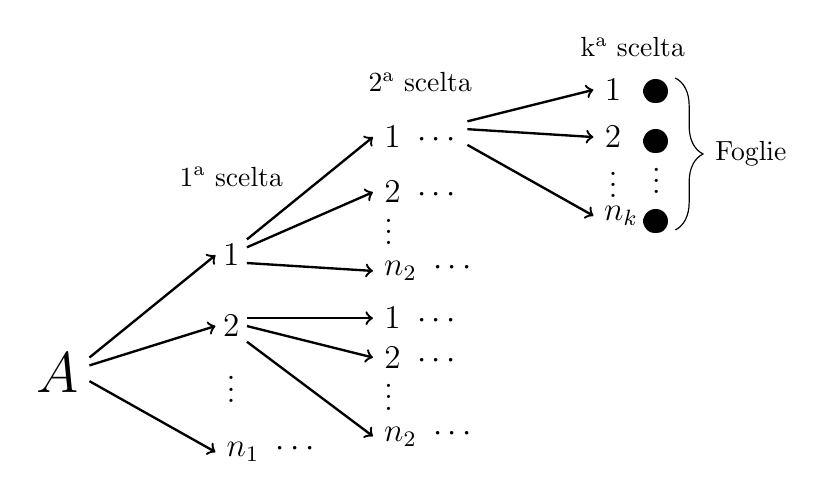
\begin{tikzpicture}
	%Parte 1
	\draw[->, line width=0.30mm] (0.4,0.2) -- (2,1.5);
	\draw[->, line width=0.30mm] (0.4,0.1) -- (2,0.6);
	\draw[->, line width=0.30mm] (0.4,-0.1) -- (2,-1);

	\node at (2.2, 2.5) {1\textsuperscript{a} scelta};

	\node at (0,0) {\huge $A$};
	\node at (2.2, 1.5) {\large $1$};
	\node at (2.2, 0.6) {\large $2$};
	\node at (2.2, -0.1) {\large $\vdots$};
	\node at (2.7, -1) {\large $n_1 \ \cdots$};

	%Parte 2
	\draw[->, line width=0.30mm] (2.4, 1.7) -- (4,3);
	\draw[->, line width=0.30mm] (2.4, 1.6) -- (4,2.3);
	\draw[->, line width=0.30mm] (2.4, 1.4) -- (4,1.3);

	\draw[->, line width=0.30mm] (2.4, 0.7) -- (4,0.7);
	\draw[->, line width=0.30mm] (2.4, 0.6) -- (4,0.2);
	\draw[->, line width=0.30mm] (2.4, 0.4) -- (4,-0.8);


	\node at (4.6, 3.7) {2\textsuperscript{a} scelta};
	\node at (4.6, 3) {\large $1 \ \cdots$};
	\node at (4.6, 2.3) {\large $2 \ \cdots$};
	\node at (4.2, 1.9) {\large $\vdots$};
	\node at (4.7, 1.3) {\large $n_2 \ \cdots$};

	\node at (4.6, 0.7) {\large $1 \ \cdots$};
	\node at (4.6, 0.2) {\large $2 \ \cdots$};
	\node at (4.2, -0.2) {\large $\vdots$};
	\node at (4.7, -0.8) {\large $n_2 \ \cdots$};

	%Foglie
	\draw[->, line width=0.30mm] (5.2, 3.2) -- (6.8, 3.6);
	\draw[->, line width=0.30mm] (5.2, 3.1) -- (6.8, 3);
	\draw[->, line width=0.30mm] (5.2, 2.9) -- (6.8, 2);

	\node at (7.3, 4.15) {k\textsuperscript{a} scelta};
	\node at (7.05, 3.6) {\large $1$};
	\node at (7.05, 3) {\large $2$};
	\node at (7.05, 2.5) {\large $\vdots$};
	\node at (7.15, 2) {\large $n_k$};

	\node at (7.6, 3.55) {\Huge\textbullet};
	\node at (7.6, 2.92) {\Huge\textbullet};
	\node at (7.6, 2.55) {\large $\vdots$};
	\node at (7.6, 1.90) {\Huge\textbullet};
	\draw [decorate,decoration={brace,amplitude=10pt,mirror,raise=4pt},yshift=0pt, line width=0.15mm]
	(7.7, 1.82) -- (7.7, 3.75) node [black,midway,xshift=1.1cm] {Foglie};
	\end{tikzpicture}
\end{figure}
Si osservi che a prescindere da quale freccia è stata percorsa alla 1\textsuperscript a scelta, la 2\textsuperscript a scelta avrà sempre $n_2$ possibilità, e così via per tutte le altre scelte.

Si riportano alcuni risultati notevoli deducibili dal principio appena riportato.

\subsubsection{Permutazioni}

\begin{defn}
	Sia dato un insieme $A$ di $n$ oggetti distinti.
	Ogni possibile ordinamento di questo insieme prende il nome di \textbf{permutazione}.
\end{defn}

Le \textit{permutazioni semplici} di $n$ elementi distinti, che differiscono per l'ordine, sono:
$$P_n = n! = n \cdot ( n-1) \cdot (n-2) \cdots 2 \cdot 1 $$

Le \textit{permutazioni con ripetizione} di $n$ elementi, dove un elemento è ripetuto $h_1$ volte, un altro $h_2$ volte, un terzo $h_3$ volte, e così via, sono:
$$P_n^{h_1,h_2,h_3, \dots}=\frac{n!}{h_1 \cdot h_2 \cdot h_3 \dots}$$

\subsubsection{Combinazioni}

\begin{defn}
	Sia dato un insieme $A$ di $n$ oggetti distinti.
	Ogni sottoinsieme di $A$ costituito da $k$ elementi, con $0 \leq k \leq n$, è detto \textbf{combinazione semplice} di $n$ oggetti di classe $k$.
\end{defn}

Le combinazioni semplici si esprimono attraverso il coefficiente binomiale:
$$C_{n,k}=\binom{n}{k}=\frac{n!}{k!(n-k)!}$$

\begin{defn}
	Sia dato un insieme $A$ di $n$ oggetti distinti.
	Ogni insieme di $k$ elementi di $A$ costituito anche da oggetti ripetuti è detto \textbf{combinazione con ripetizione} di $n$ oggetti di classe $k$.
\end{defn}

Le combinazioni con ripetizione sono:
$$C^*_{n,k}={n+k-1 \choose k}$$
Si osservi che le combinazioni non si distinguono per l'ordinamento.

È utile la conoscenza della \textbf{formula di Stiefel}:\\
\index{Stiefel, formula di}
$$ \binom{n}{k}=\binom{n-1}{k}+\binom{n-1}{k-1}, \qquad \text{oppure}\qquad \binom{n+1}{k}=\binom{n}{k-1}+\binom{n}{k}$$\\
La sua dimostrazione viene lasciata al lettore come esercizio.

\subsubsection{Disposizioni}

\begin{defn}
	Sia dato un insieme $A$ di $n$ oggetti distinti.
	Ogni possibile sottoinsieme ordinato dell'insieme $A$ di $k$ elementi prende il nome di \textbf{disposizioni semplici}.
\end{defn}

Dunque due disposizioni possono differire o per gli oggetti che contengono, o per \\* l'ordinamento degli stessi. Le  disposizioni semplici sono:
$$D_{n,k}=n	\cdot (n-1) \cdot (n-2) \dots (n-k+1) = C_{n,k} \cdot P_k$$

\begin{defn}
	Sia dato un insieme $A$ di $n$ oggetti distinti.
	Ogni possibile insieme ordinato formato da $m$ oggetti anche ripetuti dell'insieme $A$ si dice \textbf{disposizione con ripetizione} di $n$ oggetti di classe $k$.
\end{defn}

Dunque $m$ può essere sia maggiore che minore che uguale a $n$. Le disposizioni con ripetizione sono:
$$D^*_{n,k}=n^m$$

\subsection{Integrazione complessa}\label{int-complessa}
La teoria dell'integrazione per $h: (\RR^n,\Bc^n,\PP) \rightarrow (\RR,\Bc)$
si estende tale e quale per $h :(\RR^n,\Bc^n,\PP) \rightarrow (\CC,\Bc)$.
Si può infatti considerare l'unità immaginaria $i$ come una costante e scrivere la funzione complessa in forma algebrica:
$$h(x)=h_1(x)+i\cdot h_2(x), \quad \text{ con } h_1,h_2:\RR^n \rightarrow \RR$$
Ora è possibile integrare $h$ nel seguente modo:
$$\int_{\RR^n}h(x)\, \dPP=\int_{\RR^n}h_1(x)\, \dPP + i\int_{\RR^n}h_2(x) \, \dPP$$
In corsi successivi tale teoria verrà propriamente dimostrata nel dettaglio.\footnote{E invece era solo una spudorata menzogna} \\
Queste proprietà sono utili quando si utilizza la funzione caratteristica, che è, di fatto, un valore atteso (ovvero un integrale) ad argomento complesso.

\subsection{Logaritmo complesso}  \label{log-complesso}

Illustriamo ora alcune proprietà del logaritmo complesso, utile strumento per la dimostrazione del teorema centrale del limite (\ref{TCL}).

L'equazione $e^w = z$, con $z \neq 0$, ammette infinite soluzioni se l'incognita $w$ appartiene a $\CC$.
Infatti, scrivendo $z$ in forma polare, si ottiene:
\begin{align*}
	e^w = z &= \abs z e^{i \vartheta} &\text{con } \vartheta = \arg z \in [0,2\pi]\\
	& = \abs z \, e^{i (\vartheta+2k\pi)} &\text{(angoli uguali a meno di giri)} \\
	\implies w & = \log z = \ln\abs{z} + i \cdot \arg z + i\cdot 2k \pi &\text{con} \, k \in \ZZ
\end{align*}
Nell'ultimo passaggio abbiamo sfruttato la proprietà del logaritmo di un prodotto.
Si noti che con log indichiamo il logaritmo ``complesso'', mentre con ln indichiamo il normale logaritmo reale. \\
Per convenzione si sceglie la soluzione con $k = 0$; si ottiene così la funzione chiamata \textbf{logaritmo principale}:
$$\log : \CC\setminus\{0\} \to \CC, \quad z \mapsto \log z = \ln \abs{z} + i \, \arg z, \quad \text{con} \, -\pi \leq \arg z \leq \pi$$
Dunque, definendo l'insieme $D = \{z \in \CC \, : \, \abs{z} < 1\}$, la funzione $f:D \to \CC$, $f(z) = \log(1+z)$ è sempre ben definita.
La particolarità di questa funzione, che non sarà dimostrata in questo testo, è che ha lo stesso sviluppo di Taylor della sua controparte reale; quindi per $x_0 = 0$ si ha che:
$$\log(1+z) = z - \frac{1}{2}z^2 + \frac{1}{3}z^3 + \dots$$

\begin{nb}
	Anche nel caso complesso l'asintotico del logaritmo rimane invariato; infatti, sfruttando lo sviluppo di Taylor appena visto:
	%$$\frac{\log(1+z)}{z} \; \stackrel{z \to 0}{\longrightarrow} \; ?$$
	$$\frac{\log(1+z)}{z} = \frac{z + o(z)}{z} = 1+o(1) \; \xrightarrow{z \to 0} \; 1$$
\end{nb}

\subsection{Radice quadrata di una matrice} \label{sqrt-C}

Per \textbf{radice quadrata di una matrice} $C$ si intende una matrice $\sqrt{C}$ tale per cui:
$$\sqrt{C} \cdot \sqrt{C} = C $$
La trattazione sarà sviluppata solo per uno specifico tipo di matrice quadrata, in quanto il resto esula dalle necessità di questa trattazione; ma è bene tener presente che, in generale, una matrice ammette più radici quadrate.

Sia $C \in \RR^{n \times n}$ una matrice simmetrica e semi-definita positiva.
Essa è diagonalizzabile e ha tutti gli autovalori reali\footnote{``Teorema della diagonalizzazione, uno dei più importanti di tutta l'umanità''} e non negativi:
$$C=C^T \text{ e } C \ge 0 \iff \lambda_k \ge 0$$
Questo implica che $\exists \, U$ ortogonale (ovvero tale che $U^T=U^{-1}$) che verifica la seguente relazione:
$$ U C U^T = \Lambda =
\begin{bmatrix}
\lambda_1 \\
\ \ & \ddots & \ \ \\
\ \ & \ \ & \lambda_n
\end{bmatrix} \quad \text{con }\lambda_k \in \RR \enspace \forall k$$

La radice della matrice $C$ in questo caso risulta essere nella seguente forma:
$$\sqrt{C} = U^T \begin{bmatrix}\sqrt{\lambda_1} & &  \\  & \ddots &  \\  &  & \sqrt{\lambda_n} \end{bmatrix} U $$

La verifica della definizione è immediata:
\begin{align*}
	\sqrt{C} \cdot \sqrt{C} &= U \sqrt{\Lambda} U^T \cdot U \sqrt{\Lambda} U^T &\\
	&= U \sqrt{\Lambda} \sqrt{\Lambda} U^T & (U^T U = I) \\
	&= U \Lambda U^T &\text{(prop. matrici diagonali)} \\
	&= C
\end{align*}
